\documentclass{sig-alternate-2013}
\newfont{\mycrnotice}{ptmr8t at 7pt}
\newfont{\myconfname}{ptmri8t at 7pt}
\let\crnotice\mycrnotice%
\let\confname\myconfname%

\permission{Permission to make digital or hard copies of all or part of this work for personal or classroom use is granted without fee provided that copies are not made or distributed for profit or commercial advantage and that copies bear this notice and the full citation on the first page. Copyrights for components of this work owned by others than ACM must be honored. Abstracting with credit is permitted. To copy otherwise, or republish, to post on servers or to redistribute to lists, requires prior specific permission and/or a fee. Request permissions from permissions@acm.org.}
\conferenceinfo{IMC'13,}{October 23--25, 2013, Barcelona, Spain.}
\copyrightetc{Copyright 2013 ACM \the\acmcopyr}
\crdata{978-1-4503-1953-9/13/10\ ...\$15.00.\\
http://dx.doi.org/10.1145/2504730.2504736 }
\clubpenalty=10000 
\widowpenalty = 10000

\usepackage[format=plain,labelfont=bf,up,textfont=it,up,small]{caption}
\usepackage{amsmath, amssymb,alltt}
\usepackage{epsfig,url,tabularx,theorem,amsmath,amssymb,psfrag,graphics,times,subfig,multirow,color}
\usepackage{cite}
\usepackage{balance}

\newcommand{\xxx}[1]{\textcolor{red}{#1}}
\newcommand{\fp}{\vspace*{0.05in}\noindent}
\newcommand{\eg}{{\em e.g.}} 
\newcommand{\ie}{{\em i.e.}} 
\newcommand{\etc}{{\em etc. }} 
\newcommand{\ea}{{\em et al. }}
\newcommand{\etal}{{\em et al.\ }}

\renewcommand{\paragraph}[1]{\vspace*{0.1in}\noindent{\bf #1}}

\newcommand{\supsym}[1]{\raisebox{4pt}{{\footnotesize #1}}}
\newcommand{\gt}{\supsym{$\dag$}}
\newcommand{\lip}{\supsym{$\ast$}}
\newcommand{\nap}{\supsym{$\ddag$}}
\newcommand{\sk}{\supsym{$\star$}}
\newcommand{\name}{BISmark}
%\newcommand{\active}{\name-Active}
\newcommand{\passive}{\name-Passive}
%\newcommand{\groupa}{{\em Group A}}
%\newcommand{\groupb}{{\em Group B}}
\newcommand{\developed}{developed}
\newcommand{\developing}{developing}


\renewenvironment{itemize}
{\begin{list}{$\bullet$}{
    \setlength{\labelsep}{4pt}
    \setlength{\labelwidth}{3pt}
    \setlength{\rightmargin}{0pt}
    \setlength{\leftmargin}{0pt}
    \addtolength{\leftmargin}{\labelwidth}
    \addtolength{\leftmargin}{\labelsep}
}}{\end{list}}

\newtheorem{lesson}{Lesson}

%\interfootnotelinepenalty 100000

\newenvironment{pitem}{
 \begin{itemize}
 \setlength{\itemsep}{1pt}
 \setlength{\parskip}{0pt}
 \setlength{\parsep}{0pt}
}{\end{itemize}}

\begin{document}
\title{Peeking Behind the NAT: \\ An Empirical Study of Home Networks}
\author{Sarthak Grover, Mi Seon Park, Srikanth Sundaresan, \\ Sam Burnett,
  Hyojoon Kim, Nick Feamster \\ 
\affaddr{School of Computer Science, Georgia Tech}}
\maketitle

%\appendix
%\section{Appendix}


\subsection{Devices Seen}


\subsection{Link Utilization}

\begin{figure}[t]
  \begin{minipage}{\linewidth}
  \includegraphics[width=0.98\linewidth]{figures/bytesperdevice/device_utilization_entire_data}
  \caption{Device utilization for the entire two weeks period. We see that more than a third of the total traffic is by Apple(iOS) devices. This may be due to the fact that Windows/Android devices are made by multiple manufacturers.}
  \label{fig:countofdevices}
  \end{minipage}
\end{figure}

\begin{figure}[t]
  \begin{minipage}{\linewidth}
  \subfloat[Diurnal Uplink Home 5]{
  \includegraphics[width=0.98\linewidth]{figures/bitrate/diurnal-usage/5_OW4C60DED0F74B_up}
  \label{fig:diurnal-util-uplink-5}}\\
  \subfloat[Diurnal Downlink Home 5]{
  \includegraphics[width=0.98\linewidth]{figures/bitrate/diurnal-usage/5_OW4C60DED0F74B_dw}
  \label{fig:diurnal-util-downlink-5}}\\
  \caption{Diurnal pattern of link utilization for home 5}
  \label{fig:diurnal-util-5}
  \end{minipage}
\end{figure}

\begin{figure}[t]
  \begin{minipage}{\linewidth}
  \subfloat[Diurnal Uplink Home 8]{
  \includegraphics[width=0.98\linewidth]{figures/bitrate/diurnal-usage/8_OWC43DC7B0CAB6_up}
  \label{fig:diurnal-util-uplink-8}}\\
  \subfloat[Diurnal Downlink Home 8]{
  \includegraphics[width=0.98\linewidth]{figures/bitrate/diurnal-usage/8_OWC43DC7B0CAB6_dw}
  \label{fig:diurnal-util-downlink-8}}\\
  \caption{Diurnal pattern of link utilization for home 8}
  \label{fig:diurnal-util-8}
  \end{minipage}
\end{figure}

\begin{figure}[t]
  \begin{minipage}{\linewidth}
  \subfloat[Diurnal Uplink Home 11]{
  \includegraphics[width=0.98\linewidth]{figures/bitrate/diurnal-usage/11_OW4C60DEE6B01C_up}
  \label{fig:diurnal-util-uplink-11}}\\
  \subfloat[Diurnal Downlink Home 11]{
  \includegraphics[width=0.98\linewidth]{figures/bitrate/diurnal-usage/11_OW4C60DEE6B01C_dw}
  \label{fig:diurnal-util-downlink-11}}\\
  \caption{Diurnal pattern of link utilization for home 11}
  \label{fig:diurnal-util-11}
  \end{minipage}
\end{figure}  
  
\begin{figure}[t]
  \begin{minipage}{\linewidth}
  \subfloat[Diurnal Uplink Home 16]{
  \includegraphics[width=0.98\linewidth]{figures/bitrate/diurnal-usage/16_OWC43DC79DE0F7_up}
  \label{fig:diurnal-util-uplink-16}}\\
  \subfloat[Diurnal Downlink Home 16]{
  \includegraphics[width=0.98\linewidth]{figures/bitrate/diurnal-usage/16_OWC43DC79DE0F7_dw}
  \label{fig:diurnal-util-downlink-16}}\\ 
  \caption{Diurnal pattern of link utilization for home 16. Black markers denote active capacity
  estimates and green markers denote the passive measurement: max bits transferred per second in
  a minute. Units are bits per second (bps).}
  \label{fig:diurnal-util-16}
  \end{minipage}
\end{figure}

Figure ~\ref{fig:diurnal-util-5}, ~\ref{fig:diurnal-util-8}, ~\ref{fig:diurnal-util-11},
~\ref{fig:diurnal-util-16} shows that we observe a diurnal usage pattern for link activity.
Peak transfers occur in the evening and night, and some data is transferred in mornings. At
other times the link remains idle. This pattern of usage seen in half of the American homes
running \passive{} is very similar to the connectivity pattern of access points observed for
gateways in \developing{} countries such as India and China (Figure ~\ref{fig:china-availability})


\subsection{Top Domains}


\subsection{Device Utilization}

\begin{figure}[t]
  \includegraphics[width=1.05\linewidth]{figures/device_utilization}
  \caption{Device use fraction. Different markers for different homes. Color denotes type of device.}
  \label{fig:dev-util}
\end{figure}

Figure~\ref{fig:dev-util} plots the ratio of data used by a particular device in a home.

\subsection{Heartbeat}

\begin{figure}[t]
  \includegraphics[width=0.98\linewidth]{figures/outages_scatter_april}
  \caption{Red markers are developed nations, blue are developing}
  \label{fig:outage-scatter}
\end{figure}




\begin{sloppypar}
\input{abstract}

% A category with the (minimum) three required fields
\category{C.2.3}{Computer-Communication Networks}{Network Operations}[Network monitoring]
%A category including the fourth, optional field follows...
\terms{Measurement}
\keywords{BISmark, Home Networks}

\section{Introduction}

Home broadband Internet access is ubiquitous and rapidly evolving. There
are now upwards of one billion broadband Internet users
worldwide~\cite{www-internet-stats}; much of that usage is shifting away
from conventional desktops and towards mobile devices, such as laptops,
smart phones, and tablets~\cite{www-itu}.  Despite their pervasiveness,
little is known about most home networks or how people use them.

Indeed, to date, it has been surprisingly difficult to study home networks on
a large scale, because network technologies like network
address translators (NATs) present only an opaque view of the home
network to the global Internet---specifically, without a monitoring
device {\em inside} the home, traffic coming from any device in a
home network appears to all be coming from a single device.  This coarse
granularity of visibility makes it impossible to observe the usage
patterns of individual devices inside the home or observe
characteristics about other parts of a home network (\eg, the home
wireless network).  Observing home networks on a large scale requires
developing---and deploying---an always-on monitoring device in the home
that can capture information about individual devices, with the consent of
the people that live in these homes.

To better understand home networks, we developed \name{}, a custom home router, and
deployed it in more than 100 home networks in 21 countries around the world for
more than one year.  \name{} sits between the user's ISP access link and the
rest of the home network and acts as a continuous monitoring device; as a
result, it can observe all traffic entering and leaving the home network, and
can attribute traffic flows to individual devices on the network.  This
device, if permitted, can also log other types of activity, such as the number of devices on
the network at any given time and the amount of traffic that any particular
device sends to a destination (\eg, Google).  It can also independently measure
the performance of both the home wireless network and the access link.
%To better understand home networks, we developed a custom home router and
%deployed it in more than 100 home networks in 21 countries around the world for
%more than one year.  The router sits between the user's ISP access link and the
%rest of the home network and acts as a continuous monitoring device; as a
%result, it can observe all traffic entering and leaving the home network, and it
%can also attribute traffic flows to individual devices on the network.  This
%device, if permitted, can also log other types of activity, such as the number of devices on
%the network at any given time and the amount of traffic that any particular
%device sends to a destination (\eg, Google).  It can also independently measure
%the performance of both the home wireless network and the access link.
We study three aspects of home network usage:
\begin{enumerate}
\itemsep=-1pt
\item {\em Availability.} How common are Internet connectivity outages in homes,
    and how reasonable is it to assume continuous connectivity?
\item {\em Infrastructure.} What networking technologies and devices do people use
  in home networks?
\item {\em Usage.} Is the capacity of a home network sufficient for the
  growing demands of users and applications?  How does usage differ across
  individual devices in the home?  What other patterns exist?
\end{enumerate}
\noindent
%Each of these characteristics has important implications for ubiquitous
%computing.
\noindent
Although our study instruments a relatively small number of home networks,
it nevertheless offers extensive visibility into aspects of homes that were
previously opaque to researchers.  Ultimately, regulators and Internet service
providers may be able to use some of the techniques that we describe to
perform similar studies on a larger scale.  We believe that researchers,
ISPs, policymakers, and users can use the home router as a measurement
device to better understand various trends in availability,
infrastructure, and usage.  Data about availability can help regulators
determine whether ISPs are delivering the service that they are
promising to users.  Data about infrastructure (\eg, the amount of
contention in the wireless spectrum) can help ISPs better understand and
debug user performance, and can provide evidence for regulators
to release more spectrum when it becomes appropriate to do so.
Information about usage can help ISPs better provision and plan, and it
can help device designers better understand how (and when) people use
various devices.

%shorten these three paragraphs?
The {\em availability} of home broadband access networks lets developers
of applications running over edge networks understand the connectivity
conditions of a particular environment.  Our study has yielded some
surprising findings. For example, although in the Western world we often
think of broadband connectivity as ``always on'', we found examples in
China and India where users only power up their home network gateway
when they intend to use it.  We found that trends of availability
held in general: only 10\% of home networks in the \developed{} world saw
connectivity interruptions of more than ten minutes more frequently than
once every 10 days, but about 50\% of home networks in \developing{}
countries experienced such connectivity interruptions once every 3 days.
Although it is difficult from our data set to ascertain the cause for
this intermittent connectivity (\ie, it could result from power outages,
poor connectivity, or behavioral patterns), it is clear that it is not
safe to assume that Internet connectivity is highly available in certain
parts of the world.

The {\em infrastructure} of home broadband access networks lets us understand
how users construct their home networks, and what types of devices they
comprise.  We explore various questions relating to infrastructure, such as the
number of devices on each home network, and how the number of devices on these
networks varies over time with usage.  We find that in today's home network, there
are more wireless devices than wired devices in
general and this difference is greater in the \developing{} countries.  
We also find households in more \developed{} countries tend to have more devices 
compared to \developing{} countries, and
those devices are more likely to remain continuously connected to the home router.
Connectivity shows a diurnal pattern across a week;
the number of devices on the network on
weekdays typically peaks during evening hours, but on weekends device usage is
more consistent throughout the day.  The median
number of devices on a 2.4~GHz network is about five, whereas on the 5 GHz band,
the median number of devices is two.
  

The {\em usage} of home broadband Internet access can shed light on the
applications and devices that people tend to use on their home network, and the
overall utilization of these networks. We analyze 
the periodicity of usage patterns in various home networks and observe the extent
to which users saturate their access link and find that most home networks are
lightly used, and do not saturate their downstream or upstream link most of the
time.  We analyze distributions of device usage and find that users normally
have a subset of devices that they prefer to use for consuming most network
data. %mostly one device hogs all the bandwidth
We observe the diversity of domains visited and find that about 38\% of the
total volume of traffic is from a single most popular domain, among 200
whitelisted domains.

The rest of the paper is organized as follows.
Section~\ref{sec:related} overviews related work.
Section~\ref{sec:data} describes the process of collecting the various
types of data that we use in our study.  Section~\ref{sec:availability}
presents results concerning the availability of broadband access in
various home networks around the world, including the duration of
outages.  Section~\ref{sec:infrastructure} describes the characteristics
of the infrastructure in various home networks, including the number of
devices that are in the network, whether the devices are connected
via wired or wireless, and to what extent devices occupy different
ranges of radio spectrum (\eg, 2.4 GHz and 5 GHz).
Section~\ref{sec:usage} profiles the usage patterns of users in
different home wireless broadband networks and explores how usage
patterns differ across devices, and how download speed affects usage
patterns.  Section~\ref{sec:discussion} describes ongoing work and
extensions to this study and discusses some broader implications of our
results.  Section~\ref{sec:conclusion} concludes.

\section{Related Work}\label{sec:related}

We briefly review related work on home broadband networks.  We survey
work that has performed ``single shot'' measurements of home broadband
network performance and characteristics, Internet policy reports on
performance in various regions, and qualitative studies that lend
insight into how to better design home networks.

\fp {\bf Measuring home network performance.}  There has been
significant interest in measuring home and access networks, and many
previous studies have tried to measure home networks in various
ways. The studies use various methods for measuring home networks,
from running measurements remotely from servers in the Internet to
measure access link properties~\cite{Dischinger:imc2007} to running
tools on end-host
devices~\cite{DiCioccio:2012,DiCioccio2013,www-netalyzr,Kreibich2010,Sanchez2013,Chetty:2011:WMI}.
In contrast to these previous studies, we perform our measurements from
gateway routers, not end-host devices, which enables {\em continuous}
monitoring rather than one-shot measurements.  Such continuous
monitoring allows us to observe how usage patterns change over time,
both on short and long timescales, as well as to report on other
characteristics that require continuous monitoring, such as availability.
Our work builds on our own previous work~\cite{sundaresan2011}, which
uses a deployment of custom home access points that conduct a unique set
of performance measurements.  In contrast to our previous work, this study
broadly characterizes home network usage rather than focusing
on access link performance.

\fp {\bf National and regional Internet policy and measurement reports.}
Recently, there has been interest from national agencies to measure home
networks for Internet policy and regulation purposes.  The United States
Federal Communications Commission, United Kingdom's Ofcom and the
European Commission have all conducted large scale studies of access
networks in conjunction with
SamKnows~\cite{www-fcc-report,www-sk-eu,www-sk-uk}.  Benkler~\etal have
a report on broadband transitions and policies around the
world~\cite{RePEc:reg:wpaper:8}.  To date, these studies from regulatory
commissions have focused exclusively on performance of the access
network, rather than on properties of the home network itself or usage
of the home network.  The primary objective of such initiatives is to
gain an understanding of access networks to enact better policies.  They
do not perform passive monitoring of the home network.

\fp {\bf Qualitative design studies of home networks.}  There are
previous studies on understanding home networks and attempts to design
better
systems~\cite{grinter2005work,grinter2009ins,keith2011advancing,Chetty:2007:SHL,poole2008more,calvert2007moving}.
These previous studies are qualitative: they rely exclusively on human
subject interviews and analysis on human interactions to identify
problem areas and to suggest better designs.  We offer a {\em
  quantitative} complement to these studies. We analyze passive
measurement data that is automatically collected and reported, which are
in turn used to derive meaningful observations about home networks that
may not be obvious or even revealed through studies with human
subjects.  The automated nature of our data collection and monitoring
allows us to observe longitudinal behavior and usage patterns, and it may
in some cases result in more accurate data about human activity and
network usage, since many of the questions that previous studies have
asked in interviews could be more completely and accurately addressed by
measuring the network traffic itself.

Previous studies have also built tools that improve interactivity and
aid troubleshooting in a home network environment, for example
measuring and displaying bandwidth usage and throughput in a home
network~\cite{Chetty-2010,Chetty:2011:WMI}.  Our work analyzes data from
{\em existing} networks, rather than trying to deploy new tools and
observe how usage changes as a result of those tools.  We analyze a
wider variety of network features, including wired vs. wireless usage,
number of active devices, diurnal patterns, and availability.

\fp {\bf Behavioral studies of Internet usage in \developing{} countries.}
Chen \ea studied the effect of sporadic and slow connectivity on user
behavior and found a better Web interaction model for such
environments~\cite{Chen:2010:CWI}. Wyche \ea performed a qualitative
study of how Kenyan Internet users adapt their usage behavior where
Internet connectivity is a scarce resource in terms of availability,
cost, and quality~\cite{Wyche:2010:DIC}.  Smyth \ea performed a
qualitative study on sharing and consuming entertainment media on mobile
phones in urban India~\cite{Smyth:2010:TTW}.  The data that we
gathered in \developing{} countries could help
corroborate some of these studies.



%\fp{\bf Measuring home networks}~\cite{DiCioccio:2012,www-netalyzr,Kreibich2010,www-bismark,sundaresan2011,Dischinger:imc2007,Sanchez2013}\\
%\fp{\bf Understanding home networks for better design}~\cite{calvert2007moving,grinter2005work,grinter2009ins,keith2011advancing}\\
%\fp{\bf Help in interacting, troubleshooting}~\cite{poole2008more,grinter2005work,chetty2008getting,Chetty:2007:SHL}\\
%\fp{\bf Passive measurements}~\cite{DiCioccio2013}\\
%\fp{\bf Power management}~\cite{chetty2008getting,Chetty:2009:EGU}\\
%\fp{\bf Speed and bandwidth}\\

\section{Data Collection}\label{sec:data}

Home routers can observe many aspects of home networks because typically all
other devices in the home communicate both to each other and to the Internet via
the router. Over the past three years, we have deployed routers in 126 homes across
19 countries. Each router measures the quality of the upstream Internet
connection and collects limited information about device usage on the home
network. This section introduces the router platform, the data we collect from
the routers, and that data's implications for our study.

\begin{figure}[t!]
 \begin{center}
\includegraphics{figures/schematic-cacm.eps}
\caption{The BISmark home router sits directly behind
  the modem in the home network.  It collects both active and passive
  measurements.}\label{fig:bismark-deployment} 
\end{center}
\end{figure}


%\vfill
\subsection{Collection Infrastructure}

\name{} comprises gateways in the home, a centralized management and
data collection server, and several measurement servers. We have
instrumented the gateway with custom firmware that performs both passive
and active measurements. Where appropriate, the firmware anonymizes
certain aspects of the data before sending them back to the central
repository for further analysis.  Figure~\ref{fig:bismark-deployment}
shows a typical deployment in the home network, and how BISmark performs
its measurements.

\paragraph{Firmware.} \name{} is a custom home router firmware based on OpenWrt
for Netgear WNDR3800 and WNDR3700v2 routers~\cite{www-openwrt,www-netgear-3800}.
Routers have a 450~MHz MIPs processor, 16~MB of flash storage, 64~MB of RAM, an
Atheros wireless chipset, one 802.11gn radio, and one 802.11an radio.
\name{} typically replaces a household's wireless access point and connects
directly to the cable or DSL modem that provides Internet access to that
household. Because the router sits on the path between the user's home network
and the rest of the Internet, our software is uniquely positioned to capture
information about both the characteristics of network connectivity and of home
network usage (\eg, usage patterns, applications). We expected routers to remain
powered on almost all the time, since they provide the household's Internet
connectivity; however, later in this paper we show that this assumption does not
hold in several countries and regions.

\paragraph{Recruiting and deployment.} Our deployment of routers across
home networks has been organic: We have recruited most of our users by
word-of-mouth, or through targeted advertisements for specific
experiments and projects that we have run as part of our research.  For
example, the router firmware performs continuous measurements of the
performance of the home access link, which has garnered the attention of
various policy and regulatory agencies.  We have also performed smaller
recruitment efforts in various areas for a usage cap management tool
that we built on top of the firmware~\cite{kim2011communicating}.
Depending on the experiments that different users have consented to (or
not), we are able to collect different types of information.  Most users
have remained actively engaged in our experiments by virtue of the fact
that they receive a free router as a result of their participation.

%We classify the countries where we have deployed routers into two groups
%based on the GDP (Gross Domestic Product) per capita ranking in year
%2011~\cite{www-gdp}.  We call countries for whom the per capita GDP
%falls within the top 50 \groupa{}; in our deployment, these countries
%were: Switzerland, Spain, United States, Italy, Japan, Canada,
%Netherlands, Germany, Singapore, Israel, United Kingdom, Hong Kong, and
%France.  Otherwise, we define them as \groupb{}; countries in our
%deployment in this group were: India, Pakistan, Malaysia, South Africa,
%Mexico, China, Brazil, Indonesia.
We classify the countries where we have deployed routers into two groups based
on the GDP (Gross Domestic Product) per capita ranking in year
2011~\cite{www-gdp}.  We call countries for whom the per capita GDP falls
within the top 50 {\em \developed{}}; otherwise, we call them {\em \developing{}}. Table~\ref{tab:grouping}
summarizes this grouping.
%Note that we use {\em developed
%countries} for \groupa{} and {\em developing countries} for \groupb{}
%interchangeably throughout the paper.

\begin{figure}[t!]
 \begin{center}
 \frame{\includegraphics[width=\linewidth]{figures/bismark-may2013}}
\caption{The BISmark deployment as of May 2013.  Each dot indicates a
  router.  The green dots indicate routers that are currently
  reporting~(156).  Because we only use data from routers that
  consistently report data throughout the period of our study, we use
  data from 126 routers in 19 countries.  The red dots include the
  full set of routers that have ever contributed
  data~(295).}\label{fig:bismark-deployment-map}
\end{center}
\end{figure}


%%
%\begin{table}[t]
%\small
%\begin{tabular}{m{0.14\columnwidth}|m{0.60\columnwidth}|m{0.12\columnwidth}}
%{\bf Group} & {\bf Countries} & {\bf Total Routers}\\
%\hline
%{\developed{}} & {Canada, Germany, France, United Kingdom, Ireland, Italy, Japan, Netherlands,  Singapore, United States} & {90}\\
%\hline
%{\developing{}} & {India, Pakistan, Malaysia, South Africa, Mexico, China, Brazil, Indonesia, Thailand} & {36}\\
%\end{tabular}
%\centering\caption{Classification of countries based on GDP per capita.}
%\label{tab:grouping}
%\end{table}
\begin{table}[t]
\small
\begin{tabular}{m{0.30\columnwidth} m{0.10\columnwidth} | m{0.30\columnwidth} m{0.10\columnwidth}}
{\bf Developed} & {\bf Routers} & {\bf Developing} & {\bf Routers}\\
\hline
Canada & 2 & India & 12\\
Germany & 2 & Pakistan & 5\\
France & 1 & Malaysia & 1\\
United Kingdom & 12 & South Africa & 10\\
Ireland & 2 & Mexico & 2\\
Italy & 1 & China & 2\\
Japan & 2 & Brazil & 2\\
Netherlands & 3 & Indonesia & 1\\
Singapore & 2 & Thailand & 1\\
United States & 63 & {} & {}\\
\hline
Total Routers & 90 & Total Routers  & 36\\
\end{tabular}
\centering\caption{Classification of countries based on GDP per capita.}
\label{tab:grouping}
\end{table}
%%

\subsection{Data}

\begin{table}[t]
    \small
    \begin{tabular}{l|r|r|r}
        Dataset & Routers & Countries & Dates \\
        \hline
        \multicolumn{4}{c}{{\em Active measurements}} \\ \hline
        Heartbeats & 126 & 19 & October 1, 2012--April 15, 2013 \\
        Capacity & 126 & 19 & April 1--April 15, 2013 \\ \hline
        \multicolumn{4}{c}{{\em Passive measurements}} \\ \hline
        Uptime & 113 & 19 & March 6--April 15, 2013 \\
        Devices & 113 & 19 & March 6--April 15, 2013 \\ %April ?
        WiFi & 93 & 15 & Nov. 1--Nov. 15, 2012 \\
        Traffic & 25 & 1 & April 1--April 15, 2013 \\
    \end{tabular}
    \caption{Summary of data collected for this study.  With the
      exception of the Traffic data set, which is subject to privacy
    restrictions, we will publicly release all data used in this study.}
    \label{table:datasets}
\end{table}

We now summarize the data we collected from the BISmark deployment, then
describe each data set in more detail.  We will also highlight some
factors that limit the conclusions we can (or cannot) draw from our
data.  Where possible, we have released the data collected from this
study; the Capacity data (described below) is publicly available and is
also continuously updated as the routers collect new
measurements.\footnote{\url{http://uploads.projectbismark.net}} We have
released all measurements that do not have personally identifying
information (PII) (\ie, everything except the Traffic data
set).\footnote{\url{http://data.gtnoise.net/bismark/imc2013/nat}}

\subsubsection{Summary}

Table~\ref{table:datasets} summarizes the data we collected from our deployment.
\name{} routers perform both active and passive measurements. Many routers only
collect performance measurements about the router's upstream Internet connection
and basic diagnostic information about the number of connected devices; these
measurements record no personally identifying information (PII) and, as a
result, do not require written consent. In twenty-five homes
where we have explicit consent, we collect additional information about the
activity of users and devices on the home network; for those households we
clearly explained the risks of PII exposure and obtained written
consent.\footnote{Our university's Institutional Review Board (IRB) certified
all aspects of our data collection and experiments.} Engineering and consent
constraints dictated that we collect the data sets over different time periods.
We now explain each data set in more detail.

%TODO Explain anonymization procedures
% bismark-passive
%   - Overview of data collected
%   - Deployed on total of 42 routers, 34 have significant data
%   - Although we collected data for over a year, we concentrate on October
%   2012, when there were 23 active devices (21 without significant outages.)
%  - UPDATE: April 1 - 14 has 28 active devices (removing 3 since they are <100mb = 25 considered).
% bismark-active
% bismark-health
%   - uptime
%   - ethernet ports
% bdm pings

\subsubsection{Measurements}

\paragraph{Heartbeats.} Every router sends a ``heartbeat'' packet to the central
\name{} server approximately once a minute. We use this data to measure router
uptime. A heartbeat packet indicates that the router is on and online,
but a lost packet could mean a router is powered off, offline, or has
lossy connectivity to the server.  These heartbeats can be lost, and the
router makes no attempt to retransmit them. They are
nonetheless frequent enough to provide reasonable confidence
about the uptime of each \name{} router, which we analyze in
Section~\ref{sec:availability}. We consider heartbeats from 126 routers
that were on for at least 25 days between October 2012 and April 2013.

\paragraph{Uptime.} Starting in March of 2013, each router sends its uptime
every twelve hours. This data distinguishes, at coarse granularity, between
routers that are offline and those that are powered off.

\paragraph{Capacity.} Every twelve hours, each router measures the capacity of
its access link using ShaperProbe~\cite{www-shaperprobe}. In
Section~\ref{sec:saturate}, we jointly analyze the Capacity and
Traffic data to determine the extent to which users fully utilize
the capacity that their Internet service provider offers.

\paragraph{Devices.} Every hour, most routers count the number of devices
connected to their wired Ethernet ports and the number of associated clients on
each wireless frequency. This data gives a broad view of users' device usage
patterns, while still providing information at a coarse enough granularity to
preserve user privacy. Section~\ref{sec:infrastructure} uses this data to paint
a broad picture of device usage throughout the world.

\paragraph{WiFi.} Some routers collect data about the number of other access
points (APs) in the vicinity.  Each router only scans for other visible access
points in the wireless channel that it is configured for; by default, the
2.4~GHz radio is configured for channel 11, and the 5~GHz radio is configured
for channel 36. Each router attempts to scan for clients and access points every
10 minutes; unfortunately, the scanning process can sometimes cause wireless
clients to disassociate from the router,  so we reduce the scanning frequency if
the router has associated clients.

\paragraph{Traffic.} Because of potential privacy risks inherent in passively
collected data, only 53 households consented to contribute detailed information
about their devices and Internet activity. Of those, we consider data from
25 households that were active from April 1 to April 15 and exchanged at least
100~MB of traffic. To encourage 
users to consent to this data collection, we gave them access to a Web
interface that allowed them to observe and manage their usage over time and
across devices; this feature turns out to be quite useful for users who have
Internet service plans with low data caps. We collect four types of information:

\begin{enumerate}
\itemsep=-1pt
\item {\em Packet statistics.} We collect the size and timestamp of every packet
    relayed to and from the Internet. Although this data seems fairly innocuous,
    traffic analysis could in fact reveal very detailed information about user
    activity.
    %TODO risks: device identification, user behavioral patterns etc
\item {\em Flow statistics.} We collect obfuscated IP addresses and MAC
  addresses, and application ports for a sample of Internet-bound
  network flows. At surface level, this data only reveals the kinds of
  applications participants use on their Internet-enabled devices (\eg,
  HTTP, SMTP), but inference attacks similar to those on packet-level
  data are possible.
\item {\em DNS responses.} We collect a sample of A and CNAME records and
    obfuscate domain names unless they appear on a user-customizable whitelist
    of popular domain names; by default, the whitelist is the 200 most popular
    domains in the United States according to Alexa~\cite{www-alexa-us}.
\item {\em MAC addresses.} We collect the MAC addresses of devices connected to
    the router and anonymize the lower half of each address, which allows us to
    identify manufacturers without identifying specific devices.
\end{enumerate}

\noindent This data provides rich insights into user behavior inside the home.
We quantify device ownership in Section~\ref{sec:deviceVendors} and characterize
service usage in Section~\ref{sec:usage}.

%\paragraph{\passive{}} allows us to access packet headers to monitor each
%incoming and outgoing packet through the gateway and attribute it to a
%flow ({\em Passive}). Every such flow can be associated with a source and
%destination IP address, and the domain accessed by that
%packet. \passive{} maintains the router state, such as the address
%table, flow table, and domain name table (CNAME and A records), and
%detailed information about packet sizes (in Bytes) and packet time (in
%microseconds). This trace is collected and sent to the server every
%thirty seconds. Note that all MAC addresses are anonymized, and domain
%names are hashed unless they are on the user-configurable
%whitelist. \passive{} also enables us to observe device connectivity to
%each interface of the router ({\em Devices}) and the channel currently
%being used for wireless access, as well as other wireless
%characteristics, such as the number of devices associated to the access
%point and the number of access points visible from any particular region
%({\em WiFi}).  We maintain a website that indicates the availability of
%passive measurements from any of the homes where the package is
%deployed~\footnote{\url{http://sites.gtnoise.net/~sburnett/passive}}.



\subsection{Limitations}

\noindent This section discusses various limitations of our data sets.

\paragraph{Data collection may be interrupted.} Various outages and failures---both of
the routers themselves and of the collection infrastructure---introduced
interruptions in our collection.  Although we acknowledge that being able to
collect all of our data sets over the same overlapping time period would be
ideal, we needed to choose between using completely overlapping data sets from
smaller time intervals or using the largest time intervals possible for each
data set.  As such, we used overlapping time periods where possible, and in other
cases we used the largest possible time interval.

\paragraph{It is difficult to infer causes of downtime from Heartbeats.} Although we
are interested in measuring availability with the Heartbeats data, this data set
really only indicates when the BISmark router is both powered up and online.
Using this data to infer access link outages assumes that the BISmark router is
always on, but as we will see in subsequent sections, some instances of
``outages'' are in fact users who power down the router for significant portions
of the day. Additionally, these heartbeats are sent from the BISmark routers to
a server at Georgia Tech only, so a loss of heartbeats might simply result from
problems along the network path between the BISmark router and Georgia Tech.  We
assume that most persistent losses of heartbeats are due to either a failure at
the access network itself, or due to the router being powered down; we are
unable to distinguish these two cases. We started collecting uptime data
at 12-hour intervals, but this coarse granularity means we can only confirm network outages in
cases where routers are continuously powered on.

\paragraph{Privacy and ethics limit scalability.} Although we would like to observe all
passive traffic from the entire deployment, we are constrained by privacy and
ethics concerns, which compel us to restrict the size of the Traffic
data set and anonymize the data in ways that make certain types of analysis more
difficult.  For this study, we were only able to collect passive traffic traces
from 25 homes in the United States; collecting these traces requires gaining
institutional review board (IRB) approval, recruiting
users who were willing to let us collect such traces, and obtaining consent from
these users.  Even for consenting users, we anonymize a significant portion of
the passive traffic traces: We anonymize traffic to any domain name that is not
in the Alexa top 200 or otherwise explicitly whitelisted by the user, and hash
the bottom 24 bits of all MAC addresses.  This anonymization
prevents us from studying certain types of questions, such as the
characteristics of the ``tail'' of user traffic volumes.  

\paragraph{Households are not a representative population sample.} Because we
wished to minimize both capital risk and technical support investment, our
deployment is biased toward close friends, family, colleagues, and
technically-inclined volunteers in the United States and abroad. This may limit
the generality of our results, particularly those drawn from only a few routers.
Nonetheless, we believe our results shed light on important phenomena in home
networks that could be verified in later, more targeted deployments; indeed, our
ongoing research and recruitment efforts follow from data gathered on a
smaller \name{} deployment.

\paragraph{\name{} enables its 5~GHz radio by default.} Various countries have
restrictions on the use of wireless spectrum; the use of the 5~GHz spectrum on
wireless routers is only permitted in certain countries.  For the most part,
however, we do not disable the 5~GHz radio before shipping a \name{} router, and
any user who flashes their own router with the firmware that we have published
on the Web may have the 5~Ghz spectrum enabled by default. Therefore, although
it might be interesting to explore the use of 5~GHz spectrum in countries where
it is not legal, the way that we have deployed our routers necessarily biases
our data set and does not allow us to answer this question accurately.
%\pagebreak{}
%%%%%%%%%%%%%%%%%%%%%%%%%%%%%%%%%%%%%%%%%%%%%%%%%%%%%%%%%%%%


%\begin{table}
%    \small
%    \begin{tabular}{l|l}
%        Type of data & Examples \\ \hline
%         Link header & MAC addresses (Ethernet), Signal strength (WiFi) \\
%      Network header & Network addresses (IP) \\
%    Transport header & Port numbers (TCP, UDP) \\
%  Application header & Domain names (DNS), URLs (HTTP) \\
%    Application data & Page contents (HTTP), E-mails (SMTP) \\
%    \end{tabular}
%    \caption{Several kinds of data are available to passive measurement tools
%    running on \name{}{} routers. Risks to privacy increase with the amount
%    of data collected.}
%    \label{tab:passive-data}
%\end{table}
%
%Table~\ref{tab:passive-data} summarizes the data available to passive
%measurement tools on home routers. There are no guidelines for what is
%absolutely safe to collect, since attackers could always infer meaning from
%seemingly meaningless information. For example, researchers showed it is
%possible to infer the language and sometimes even contents of encrypted VoIP
%calls\cite{white2011, wright2007}; Sun \ea{} demonstrated how to identify URLs
%from Web browsing sessions using only packet sizes and
%timestamps~\cite{sun2002}. Participants must trust that researchers to use
%collected data only for its stated purpose and to prevent disclosure to
%untrusted third parties. Whether participants consent to a particular type of
%data collection varies between individuals depending on their knowledge and
%personal history.
%
%\subsubsection{\name{}-Passive}
%
%We built a passive measurements application, \passive{}, to discover how people
%use devices in their homes to access services on the Internet. Two research
%projects use data we collect and motivate the scope of data collection. One
%project builds profiles of traffic statistics of each device for a new class of
%network anomaly detector. Because the new class of anomaly detector is
%specifically designed to work without packet payloads, our tool doesn't need to
%collect packet payloads; doing so would unnecessarily increase privacy risks.
%Other other hand, another project using the data infers real-world events (\eg,
%sleeping, working, eating) from network-level data using time series analysis.
%This project could make use of arbitrary amounts of collected data.  The amount
%of data we collect is determined by users' willingness to divulge the data and
%the feasibility of collecting and transferring the data without disrupting the
%home network's normal operation.  The remainder of this section discusses
%\passive{} and the design tradeoffs we make to balance user privacy and
%convenience against measurement quality.  \xxx{Reframe these tradeoffs using
%    terms we introduce in previous sections.}
%
%     - What data we collect
%         - Packet sizes and timestamps
%         - Flow 5 tuples (unidirectional) w/ hashed IP addresses, correlated to
%             packet data.
%         - DNS responses (A and CNAME packets), correlated to packet data.
%         - MAC addresses for all devices
%         - Augmenting with ESM
%
%\fp{\bf Data collected.} \passive{} collects three kinds of network data:
%
%\begin{enumerate}
%\item {\em Packet statistics.} We collect the size and timestamp of every
%    packet relayed to and from the Internet. As explained earlier, although
%    this kind of data seems fairly ``safe'', in certain circumstances it can
%    in fact be used to reveal very detailed information about user activity.
%\item {\em Flow statistics.} We collect obfuscated IP addresses and MAC
%    addresses, and application ports for every Internet-bound network flow.  At
%    surface level, this data only reveals the kinds of applications participants
%    use on each of their Internet-enabled devices (\eg, HTTP, SMTP, etc.), but
%    inference attacks similar to those on packet-level data are possible.
%\item {\em DNS responses.} We obfuscate domain names unless they appear on a
%    user-customizable whitelist of popular domain names; by default, the
%    whitelist is the 200 most popular domains in the United States according to
%    Alexa~\cite{www-alexa-500-us}.
%\end{enumerate}
%
%\noindent We augment the network data with user diaries; each user has kept a
%log of when he is at home, when he is asleep, and which devices and services he
%uses and when. The diary provides a limited degree of ground truth to calibrate
%the passive measurements data for the activity sensing project.
%
%\fp{\bf Collection volume.} Along with addressing privacy concerns, \passive{}
%must operate without disrupting the home network's normal operation. Similarly
%to active measurements, this means that collecting data shouldn't impact the
%forwarding performance of the \name{}{} router, and uploading encrypted
%measurements data to our server shouldn't saturate the user's uplink. We take
%several steps to address these constraints.
%
%On our target platform, the Netgear WNDR3700v2, we find that RAM is the most
%constrained resource.  \passive{} uses fixed-size buffers for storing collected
%measurements; we drop all measurements that exceed these buffers. Even when
%using a significant fraction of the router's limited RAM, \passive{} drops 2\%
%of packets and 1\% of flows on some routers with high-capacity access links.
%
%After data is recorded we upload it to a storage server, because storage space
%on the router itself is very limited. We must take care not to saturate the
%user's uplink, so we only collect data to and from the Internet, not traffic
%between devices in the home. This ensures the amount of data collected is
%proportional to the capacity of the user's access link. High-bandwidth transfers
%within the home could cause \passive{} to either drop or upload excessive
%amounts of data over a short period. We also compress the data we transmit and
%use label substitution to avoid sending duplicate flow data.

\section{Availability}\label{sec:availability}

%Internet connectivity in developed countries could be considered an ``always
%on'' resource. In this section we look at the availability of Internet
%connectivity. 

We first study the extent to which Internet connectivity was available across
the home broadband networks in our deployment, and whether any remarkable
availability or usage patterns emerged.  We observe the frequency and duration
of downtime across the deployment and the extent to which these characteristics
differ between home networks---we explore differences between
\developing{} and \developed{} countries (and specifically, how downtime
characteristics vary according to a country's GDP), as well as usage
patterns that are unique to individual homes.

We measure the availability of
Internet connectivity by recording periodic heartbeat messages
which every router sends to our central server approximately once per minute. The
arrival of a heartbeat signifies that the router is up and connected to
the Internet.  We define {\em downtime} as any gap in the heartbeat
logs that lasts longer than ten minutes.  The absence of a heartbeat
could signify that the router is offline, has been shut down or
rebooted, or that the heartbeat was lost.  For reboots the
router usually comes back up within a few minutes. In some cases, we can
positively verify downtimes caused by powered off routers using the Uptime data set. All results in
this section are based on the Heartbeats and Uptime data sets, as described in
Section~\ref{sec:data}.  Table~\ref{tab:availability-results} summarizes
a few of the more interesting results.


\begin{table}[t]
\begin{small}
\begin{tabular}{|p{2.6in}l|}
\hline
& \\

Developed countries experience far less frequent extended downtime than
\developing{} countries: The median time between downtime in \developed{}
countries is more than a month while in \developing{} countries it is
less than a day. & \S\ref{sec:uptime}, Fig.~\ref{fig:cdf-outages} \\ & \\
%
The two countries in our deployment with the most frequent downtime are those with
the lowest per-capita GDP (India and Pakistan). & \S\ref{sec:uptime},
Fig.~\ref{fig:outages-scatter} \\ & \\
%
In some cases in \developing{} countries, broadband connectivity is not
``always on'' because users only turn on their routers to use the
Internet. & \S\ref{sec:avail-case}, Fig.~\ref{fig:china-availability} \\ & \\
\hline
\end{tabular}
\end{small}
\caption{Highlights of Section~\ref{sec:availability} results.}
\label{tab:availability-results}
\end{table}


\subsection{How reliable is home broadband access?}\label{sec:uptime}

We study the ``uptime'' of home broadband Internet access across home
networks in our deployment, in terms of the frequency and duration of
downtime.  We also explore the extent to which these characteristics vary
by country.

\begin{figure}[t]
  \begin{minipage}{\linewidth}
  \includegraphics[width=0.98\linewidth]{figures/cdf_avg_downtimes_per_day_clean}
  %\includegraphics[width=0.98\linewidth]{figures/cdf_avg_outages_per_day_v2}
%  \subfloat[For \groupa{}, 20\% of users see an outage more than once every 10 days]{
%  \includegraphics[width=0.98\linewidth]{figures/cdf_outage_num_rc}
%  \label{fig:cdf-outage-developed}}\\
%  \subfloat[For \groupb{}, about 50\% of users see an outage every 3 days]{
%  \includegraphics[width=0.98\linewidth]{figures/cdf_outage_num_nsrc}
%  \label{fig:cdf-outage-developing}}
  \end{minipage}
  \caption{Average number of downtimes per day that last at least ten
    minutes. Developed countries experience far fewer downtimes per day than 
developing countries.}
  \label{fig:cdf-outages}
\end{figure}


\begin{figure}[t]
  \begin{minipage}{\linewidth}
  \includegraphics[width=0.98\linewidth]{figures/cdf_downtime_duration_clean}
  %\includegraphics[width=0.98\linewidth]{figures/cdf_median_outage_duration_clean}
  %\includegraphics[width=0.98\linewidth]{figures/cdf_outage_duration}
  \caption{Downtime duration for developing and developed
    countries. The median downtime duration 
   is similar, but as we see in Figure~\ref{fig:cdf-outages}, 
   developing countries see downtime much more frequently.}
  \label{fig:cdf-outage-duration}
  \end{minipage}
\end{figure}


\begin{figure}[t]
  \begin{minipage}{\linewidth}
  \includegraphics[width=0.98\linewidth]{figures/num_downtimes_scatter_clean_v2}
  %\includegraphics[width=0.98\linewidth]{figures/num_outages_scatter_clean}
  %\includegraphics[width=0.98\linewidth]{figures/outages_scatter_april}
  \caption{The median number of downtimes across homes in each
    country during October 2012 -- April 2013 vs. the GDP of the country where that home
    network was located. The marker size is proportional to the median downtime duration
    in that country. The vertical line separates
    developing and developed countries. We show only countries with
    at least three routers deployed.}
  \label{fig:outages-scatter}
  \end{minipage}
\end{figure}



\paragraph{Frequency of downtime.}  Figure~\ref{fig:cdf-outages} shows a
distribution of the downtime over six months, for both \developed{} and
\developing{} countries; we show a distribution of the average number of
downtimes per day for each network, where downtime is defined as an interruption
in connectivity of ten minutes or longer.  As expected, the home networks in
\developing{} countries sustain substantially more downtime compared to those in
\developed{} countries. The median duration between downtimes for networks in
\developed{} countries is more than a month, whereas for \developing{}
countries, the median duration between downtimes is less than a single day.

\paragraph{Duration of downtime.}
Figure~\ref{fig:cdf-outage-duration} shows a cumulative distribution function
of the downtime durations for both \developing{} and
\developed{} countries.  The plot shows that the median downtime duration 
is approximately 30 minutes, and that downtime in \developing{}
countries tend to last longer.  Downtime sometimes lasts several days.  

\paragraph{Downtime characteristics vs. per-capita GDP.}
Figure~\ref{fig:outages-scatter} shows a scatter plot of the median
number of downtimes experienced by home networks in each country vs. the
{\em per-capita GDP} for that country in U.S. dollar equivalent (\ie,
the purchasing power parity)~\cite{www-imf-gdp} for countries with at
least three deployed routers.  The vertical line divides
nine \developing{} from eleven \developed{} countries.  Although
there is no discernible difference between any of the \developing{} and
\developed{} countries in terms of the median number of downtimes, the two
countries with the lowest per-capita GDP in our deployment---India and
Pakistan---experienced significantly more downtime during October 1, 2012 -- April 15,
2013. A home network in Pakistan experienced nearly two downtimes lasting
at least ten minutes every day.\footnote{These characteristics are are
  based on data from about 12 routers in India and about five routers in
  Pakistan for October 1, 2012 -- April 15, 2013.  In general, some country data from
  this scatter plot may be inconclusive, due to the small number of
  countries from which we collect data, but the trend appears to hold
  for at least the poorest countries.}


\subsection{Case Study: Router as Home Appliance}\label{sec:avail-case}

\begin{figure}[t]
    \begin{minipage}{\linewidth}
    \subfloat[This household never intentionally turns off its router,
    which is typical of routers in developed countries.]{
        \includegraphics{figures/developed_availability}
        \label{fig:developed-availability}
    }

    \subfloat[This household often turns off its router when not using it. The
    router is available briefly in evenings and during weekends.]{
        \includegraphics{figures/china_availability}
        \label{fig:china-availability}
    }

    \subfloat[This household's access link experienced sporadic ISP outages for
    several days in April 2013. Although the router was continuously powered on,
we label this as downtime.]{
        \includegraphics{figures/comcast_availability}
        \label{fig:comcast-availability}
    }
    \caption{Examples of different modes of router availability. The thick
        horizontal green lines indicate intervals when the router is {\em
        available}. For reference, dark shaded regions indicate nighttime hours and
        lighter shaded regions indicate weekend daylight hours.}
    \end{minipage}
\end{figure}


In addition to general trends, we also discovered some interesting cases of
availability and usage patterns.  We observed that in the United States, most
users leave their routers powered on all of the time.
The median US user has his router on 98.25\% of time in the measured time period.
Router availability in these homes resembles Figure 6a.
In contrast, 
{\em home broadband is not ``always on'' in the developing world.}
As a comparison, median routers in India and South Africa stay on only for 76.01\% and 
85.57\% of the time, respectively.  
We observed cases where users powered their router on for specific
time periods when they were using the Internet, much as someone would use any
other appliance. 
We envision multiple
possible reasons for this disparity. One reason could be {\em behavioral patterns}: in some
cases, we can observe specific patterns where users power down their
router when they are not actively using it (because of data usage caps
imposed by certain ISPs).  For example,
Figure~\ref{fig:china-availability} shows one Chinese household that
consistently keeps its router off except during the early
evening. During the weekend, the router is on for longer periods,
presumably with increased activity.  
Another reason could be {\em poor
  connectivity}, such as high loss or network outages caused by
congestion, overload, or even poor infrastructure or
equipment, as is possibly the case for the home network in
Figure~\ref{fig:comcast-availability}.

\section{Infrastructure}\label{sec:infrastructure}

This section examines the {\em infrastructure} that people in home
networks use to access the Internet. We look at the typical composition
of devices in home networks, be they wired or wireless, and
operate either in the 2.4~GHz or the 5~GHz
wireless spectrum. Table~\ref{tab:infrastructure-results} summarizes the main
results from this section.

%\begin{itemize}
%\item Todo - CDF of fraction of times devices seen (developed v developing countries)
%\end{itemize}

\begin{figure}[t]
%\centering
%\includegraphics[width=0.9\linewidth]{figures/count_of_devices}
%\centering  \includegraphics[width=\linewidth]{figures/health/region_stat/region_stat_cdf}
\centering  \includegraphics{figures/health/region_stat/region_stat_cdf}
  \caption{Number of devices in each home network.  More than half of the homes
  have at least five devices. Each home network has seven devices on average.} 
  \label{fig:countofdevices}
\end{figure}



%unique devices median, ignore devices on 5GHz in countries where 5GHz is not allowed
\begin{figure}[t]
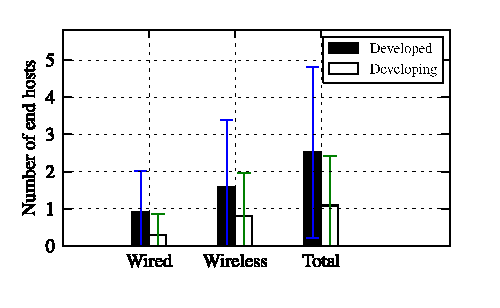
\includegraphics{figures/health/region_stat/region_stat_combined}
  \caption{Average number of devices connected to the access point at any time
  with error bars showing the standard deviation.  We see that there are more
  wireless devices in both regions. Developed has more devices overall, and
  an even greater number of wired devices.}
  \label{fig:avg_by_region}
\end{figure}


\begin{figure}[t]
  \includegraphics{figures/health/region_stat/region_stat_combined_wl}
\caption{Average number of wireless devices connected at any given time per
spectrum with error bars showing the standard deviation.  There are
significantly more devices on 2.4~GHz than on 5~GHz.}
  \label{fig:avg_spectrum_by_region}
\end{figure}


\subsection{How many devices?}\label{sec:devices}

\fp {\bf More devices in \developed{} countries.}
%TODO: might change with Joon's new plots
Figure~\ref{fig:countofdevices} shows a CDF of the number of devices
seen in each home; twenty percent of networks had at least
two unique devices, and more than half of homes had at least five
unique devices.
Figure~\ref{fig:avg_by_region} details the number of devices for
\developed{} and \developing{} countries. 
Developed countries have, on average, one more device connected to
the access point at any given time than \developing{} countries.
%This discrepancy is more pronounced in wired devices than in wireless.
%Households in \developed{} countries tend to have more devices or
%``gadgets'' in use, especially wired (it is possible that devices such as gaming consoles
%and entertainment devices, which tend to be wired, are responsible for this discrepancy).
All in all, households in countries with higher economic standards tend
to have more devices in their network, and this number is more pronounced for
wired devices. We assume this is because gaming consoles (\eg, XBox,
Playstation, Wii) or entertainment devices (\eg, Apple TV, Google TV,
Squeezebox) are more common in \developed{} countries.

\begin{table}[t!]
\begin{small}
\begin{tabular}{|p{2.6in}l|}
\hline
& \\
In \developed{} countries, 43\% of home networks have at least one
always-on wired device; only 12\% of home networks in \developing{}
countries have such as device. & \S\ref{sec:devices},
Tab.~\ref{tab:always-conn} \\ & \\ 
%
The 2.4~GHz spectrum is significantly more crowded; the median number of
devices seen on the 2.4~GHz spectrum is five, whereas on the 5~GHz band,
the median number of devices is two. & \S\ref{sec:spectrum},
Fig.~\ref{fig:cdf-devices} \\ & \\ 
%
The median number of access points seen from a home network in
\developed{} countries is about 20; in contrast, home networks in
\developing{} countries see a median of about two access points &
\S\ref{sec:spectrum}, Fig.~\ref{fig:cdf-aps} \\ & \\ 
\hline
\end{tabular}
\end{small}
\caption{Highlights of Section~\ref{sec:infrastructure} results.}
\label{tab:infrastructure-results}
\end{table}


\if 0
%%
\begin{table}[t]
\small
\begin{tabular}{ |r|r| }
  \hline
  {\bf Number of Devices} & {\bf Fraction of Homes} \\
  \hline
  at least 3 & 28/28 (100\%) \\
  6 & 23/28 (82\%) \\
  9 & 16/28 (57\%) \\
  12 & 8/28 (29\%) \\
  15 & 5/28 (28\%) \\
  18 & 2/28 (7\%) \\
  \hline
\multicolumn{2}{|r|}{Average: 9 devices} \\
  \hline
\end{tabular}
\centering\caption{Number of devices present per each
  household. \xxx{make this a CDF}}
\label{tab:countofdevices}
\end{table}
%%
\fi

\fp {\bf More ``always-connected'' devices in \developed{} countries.}
Table~\ref{tab:always-conn} shows the number of households that have at least
one wired or wireless device that never disconnects from the home gateway router
for over five weeks and its percentage against the total number of households.
The portion of households that have at least one ``always-connected'' device in
\developing{} countries is significantly lower than for \developed{} countries.
Media entertainment boxes are an example of a wired device that
never disconnects from the router, and a wireless VoIP phone is an
example of an ``always-on'' wireless device.  Some households may never
turn off their desktop or laptop.
Although we do not explore the reasons for such connectivity in depth,
we assume that households in \developing{} countries tend to power off devices
when not in use, possibly to minimize electricity 
or data usage.  Unexpected and frequent power
outages in these countries also affect device connectivity.
%%
%TODO: Table 3: Show graphs? (column 3) - parameters to be explored; maybe per 12 hour or something
\begin{table}[t]
\small
\begin{tabular}{m{0.15\columnwidth}|m{0.1\columnwidth}|m{0.26\columnwidth}|m{0.26\columnwidth}}
{\bf Group} & {\bf Total houses} & {\bf Houses with always-connected wired device} & {\bf Houses with always-connected wireless device}\\
\hline
{\developed{}} & {79} & {34 (43\%)} & {16 (20\%)}\\
{\developing{}} & {34} & {4 (12\%)} & {4 (12\%)}\\
\end{tabular}
\centering\caption{Number of households that has one or more wired or wireless device which
never disconnects from the home gateway router for over five weeks.}
\label{tab:always-conn}
\end{table}
%%



%there would
%be much less 5~GHz-capable devices than 2.4~GHz %as it is only built in the
%latest wireless devices today.

%\fp {\bf More devices used in developed countries.}
%The Figure shows that developed countries tend to have more devices (wired and
%wireless) attached in general when compared to developing countries. This can
%be caused by many reasons. 



\subsection{Wired or wireless?}

\fp {\bf More wireless than wired.}
Figure~\ref{fig:avg_spectrum_by_region} shows the average number of wired and wireless
devices attached to (and associated with) the home router 
over two
weeks, measured hourly, for \developed{} and \developing{} router groups. 
There are generally more wireless devices than wired devices.
Although this observation could reflect limitations of the router, which has only four available wired ports,
  the average number of wired ports used is
less than one in both groups; this shows that many households use wireless
even though wired connections generally
provide better throughput, latency, and stability.  This result also confirms the trend of moving away from wired
communication~\cite{www-itu} and towards primarily using wireless devices access the
Internet. For many households, wireless technology has
developed to the point where it is good enough for day-to-day Internet usage, and wired communication has little more to offer.

On the other hand, our results also suggest that wired devices are still in fairly widespread
use in some homes.  Chetty \ea stated that home users still desire wired communication
for reliability, speed, and security~\cite{Chetty:2007:SHL}.  Due
to the physical constraint of wired communication (\ie, 
cabling) devices using wired ports are likely stationary ones such as
desktop machines, network printers or media entertainment gadgets like
Apple TV. Even in homes with wired devices, our analysis suggests that a typical home gateway router
could likely suffice with only two ports. Surprisingly, only a few
households use all four Ethernet ports (9\% for both \developed{} and \developing{}
countries).
%There are few households that actually max out their wired ports
%($4$ in total) on the home gateway router.


\subsection{How much is each spectrum used?}\label{sec:spectrum}

Spectrum contention is an important problem in home wireless
networks. Many devices talking to many access points in the vicinity
causes contention and interference problems, which in turn reduces the
available bandwidth of the wireless channel. Our results confirm that
the 2.4~GHz spectrum is quite crowded, especially in \developed{}
countries, which could create bottlenecks as access link throughputs
continue to increase.  The 5~GHz spectrum, on the other hand, is less
crowded (at least for now).

\fp {\bf Wireless spectrum usage.}
Figure~\ref{fig:avg_spectrum_by_region} shows that there are more
devices active on the 2.4~GHz spectrum than on the 5~GHz spectrum at any
given time. This phenomenon may result from the fact that dual-band
devices are more expensive, and single-band devices default to the more
popular 2.4~GHz spectrum. Phones are equipped almost exclusively with
only 2.4~GHz radios.  Figure~\ref{fig:cdf-devices} shows a CDF of the
total number of {\em unique} devices seen per household. We see that the
median number of devices on the 2.4~GHz spectrum is five, while the
median number of devices on the 5~GHz spectrum is two.

We see a similar trend in the number of other access points seen on both
spectrums. The median number of other access
points is only about one device in the 5~GHz spectrum, while it is higher
for the 2.4~GHz spectrum, as expected.
Figure~\ref{fig:cdf-aps} shows a CDF
of the total number of unique access points seen per household. 
Scanning is done only in the channel the access point is configured in
(channel 11 for 2.4~GHz by default, though the user can configure it),
so this does not tell us all
the access points available, but it does tell us how likely it is
that interference occurs due to competing access points. We see that
the 2.4~GHz spectrum is more densely occupied in \developed{} countries,
and interestingly, we see
that there are two modes in both sets; either there are
very few access points in that channel or there are a lot (more than ten in \developed{}
and more than three in \developing{} countries).
%We hypothesise that this is
%an indication of users living in apartments versus those in homes.
%Figure~\ref{fig:avg_spectrum_by_region} shows that there are more devices
%active on the 2.4~GHz spectrum than 5~GHz at any given time. This seems mostly
%due to the fact that dual band devices are more expensive, and single-band
%devices default to the more popular 2.4~GHz spectrum. Phones are equipped
%almost exclusively with only 2.4~GHz radios.  Figures~\ref{fig:cdf-2-devices}
%and~\ref{fig:cdf-5-devices} show the CDF of the total number of unique devices
%seen per household.
%
%Figures~\ref{fig:cdf-2-aps} and~\ref{fig:cdf-5-aps} show the CDF
%of the total number of unique access points seen per household. The 
%scanning is done only in the channel the access point is configured in
%(channel 11 for 2.4~GHz and 36 for 5~GHz), so this does not tell us all
%the access points available, but it does tell us how likely it is 
%that interference occurs due to competing access points. We see that
%the 2.4~GHz spectrum is more densely occupied, and interestingly, we see
%that there are two modes in the developed countries; either there are
%very few access points in that channel or there are a lot ($>$ 10).
%Also, as expected, the spectrum is more polluted in the developed countries.
  
%About 10\% of the devices in our data set are dual-band capable.
%Figure~\ref{fig:cdf-frac-5} shows the fraction of time such devices use the
%5~GHz spectrum. We expected to see that devices almost exclusively use either
%one or the other (based on initial configuration), but surprisingly there seems
%to be no real pattern; devices are almost equally likely to stick to one
%spectrum as they are to hop between different spectrums.



%fig 7: TODO any other way to show this figure
\begin{figure}[t]
  \begin{minipage}{\linewidth}
  \includegraphics{figures/cdf_clients_all}
  \caption{Number of unique devices seen on the two wireless
    spectrums. The median is about five devices on 2.4~GHz and two
    devices on 5~GHz.} 
  \label{fig:cdf-devices}
%  \subfloat[Median number of devices seen on 2.4~GHz spectrum is 5]{
%  \includegraphics[width=0.98\linewidth]{figures/cdf_clients_wlan0}
%  \label{fig:cdf-2-devices}}\\
%  \subfloat[Median number of devices seen on 5~GHz spectrum is 2 (among homes which see devices in the 5 spectrum)]{
%  \includegraphics[width=0.98\linewidth]{figures/cdf_clients_wlan1}
%  \label{fig:cdf-5-devices}}
%  \caption{Number of devices seen on the two spectrums}
%  \label{fig:cdf-devices}
  \end{minipage}
\end{figure}

%fig 6
\begin{figure}[t]
  \begin{minipage}{\linewidth}
  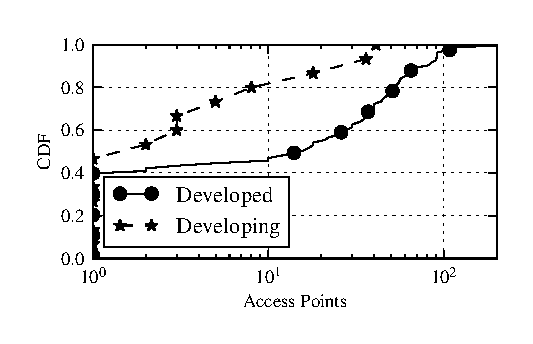
\includegraphics{figures/cdf_aps_all}
  \caption{Number of access points seen on the 2.4~GHz spectrum in \developed{} and \developing{} countries. There are many more access points visible in \developed{}, where we see modal behavior with either very few or a lot of neighboring access points.}
  \label{fig:cdf-aps}
%  \subfloat[Median number of APs seen on 2.4~GHz spectrum is about 10 in developed countries]{
%  \includegraphics[width=0.98\linewidth]{figures/cdf_aps_wlan0_rc}
%  \label{fig:cdf-2-aps-rc}}\\
%  \subfloat[Median number of APs seen on 2.4~GHz spectrum is 2 in developing countries]{
%  \includegraphics[width=0.98\linewidth]{figures/cdf_aps_wlan0_nsrc}
%  \label{fig:cdf-5-aps-nsrc}}
%  \caption{There is a clear bimodal pattern in the number of APs seen}
%  \label{fig:cdf-2-aps}
  \end{minipage}
\end{figure}




%TODO this paragraph doesn't seem important for IMC

%% \paragraph{How many devices are capable of dual band?}
%% About 10\% of the devices in our data set are dual-band capable.
%% Figure~\ref{fig:cdf-frac-5} shows the fraction of time such devices use the
%% 5~GHz spectrum. We expected to see that devices almost exclusively use either
%% one or the other (based on initial configuration), but surprisingly there seems
%% to be no real pattern; devices are almost equally likely to stick to one
%% spectrum as they are to hop between different spectrums.
%% %TODO: implication may change with new plots

%% %TODO: is this valid? need to redo plot
%% \begin{figure}[t]
%% \includegraphics[width=0.98\linewidth]{figures/cdf_frac_5_usage}
%% \caption{Among dual-band devices, there is no discernible preference for either
%% 2.4 or 5~GHz}\label{fig:cdf-frac-5}
%% \end{figure}

%\subsection{Usage patterns of wireless devices}
%Figure~\ref{fig:diurnal-all} shows the usage patterns of all wireless devices
%across a day, broken down into weekday (Monday-Friday) and weekend. We see that
%there is a clear diurnal pattern in the number of unique devices seen at
%various times of the day during the weekday. Usage peaks during the evenings,
%and troughs during the afternoons. The wireless devices could be either laptops
%or cellular devices. We see that the number of devices dips only slightly at
%night (compared to the dip during the day), so it's most likely to be cellular
%devices, as laptops are more likely to be switched off at night. On weekends,
%we see no discernible diurnal patterns.

%\begin{figure}
%  \begin{minipage}{\linewidth}
%  \subfloat[Median number of APs seen on 5~GHz spectrum is about 2 in developed countries]{
%  \includegraphics[width=0.98\linewidth]{figures/cdf_aps_wlan1_rc}
%  \label{fig:cdf-5-aps-rc}}\\
%  \subfloat[Median number of APs seen on 5~GHz spectrum is 1 in developing countries]{
%  \includegraphics[width=0.98\linewidth]{figures/cdf_aps_wlan1_nsrc}
%  \label{fig:cdf-5-aps-nsrc}}
%  \caption{The number of APs seen in 5~GHz is much lower than on 2.4~GHz}
%  \label{fig:cdf-5-aps}
%  \end{minipage}
%\end{figure}
%
%
%
%\begin{figure}[t]
%\includegraphics[width=0.98\linewidth]{figures/cdf_frac_5_usage}
%\caption{Among dual-band devices, there is no clear preference for 2.4 or 5}\label{fig:cdf-frac-5}
%\end{figure}

\subsection{Which device vendors are most common?}\label{sec:deviceVendors}

For the 25 homes in the United States in the Traffic data set, we observed the
frequency of various types of devices connected to the home network. When
collecting the Traffic data set, we obfuscate the bottom 24 bits of the MAC
addresses of all devices seen by the gateway. The first 24 bits allow us to look
up the manufacturer, and though this does not always tell us if the device is a
phone, tablet, or laptop, it still provides us enough information to distinguish
network gateways from smart devices and wireless cards.

\begin{figure}[t!]
%filtered to devices atleast > 100 KB data in 15 days -- misses the printers
\includegraphics[width=\linewidth]{figures/devices_seen_filtered}	
%\includegraphics[width=\linewidth]{figures/devices_seen_v2}			%unfiltered
\caption{The number of devices seen in the Devices data set across
  all homes in the Traffic data set (25 homes in the United States).
  We only considered devices which transferred at least 100 KB. }
 \label{fig:manufacturer}
\end{figure}



Based on passive monitoring of 25 homes, Figure~\ref{fig:manufacturer} plots the
device types seen in the Traffic data set. We have removed all
references to Netgear originating from our BISmark routers. The most common device was manufactured by Apple, followed by Intel.  Other Samsung and smart phones
were also reasonably common.\footnote{ The {\em
  Printer} manufacturer was an Epson. {\em Hardware} includes Giga-Byte
and Microchip.  {\em VoIP} is a UniData device.  {\em Internet TV}
includes Roku, TiVo, and ASRock home theatres.  {\em Wireless Card}
includes AzureWave and GainSpan. {\em Gaming} includes Nintendo and
Mitsumi (which manufactures controllers for Playstations, Xbox, and
Wii).  Microsoft (possibly Xbox) is shown separately. Gateway includes
TP-Link, Realtek, Liteon, D-Link, Cisco-Linksys, Belkin, and Askey. {\em
  Smart Phones} includes HTC, LG, Motorola, Nokia, and a confirmed
Samsung Galaxy S II (Murata Inc.).  Other Samsung devices, including
phones and tablets, are shown separately.  {\em Original Device
  Manufacturers (ODMs)} include Compal, Hon Hai Precision, Quanta,
Universal Global Systems, Winstron Infocomm. Misc. includes Polycom (a
telecom product manufacturer), Prolifix (which makes Internet-enabled
thermostats), and Pegatron (which manufactures a variety of products
including notebooks, laptops to gateways).}  We recently started
gathering Traffic data in several \developing{} countries, so we will soon
be able to compare the distribution of device manufacturers in \developed{}
and \developing{} countries.

\begin{figure}[t]
  \begin{minipage}{\linewidth}
  \subfloat[Weekday usage is diurnal.]{
  \includegraphics{figures/clients-diurnal-weekday-all}
  \label{fig:weekday-diurnal-all}}\\
  \subfloat[Usage on weekends is more constant.]{
  \includegraphics{figures/clients-diurnal-weekend-all}
  \label{fig:weekend-diurnal-all}}\\
  \caption{Diurnal effect on wireless device usage. There is a clear
    weekday diurnal effect on the number of devices online.}
  \label{fig:diurnal-all}
  \end{minipage}
\end{figure}

\begin{figure}[t]
  \begin{minipage}{\linewidth}
  \subfloat[Upstream traffic, and the measured upstream capacity.]{
  \includegraphics[width=0.98\linewidth]{figures/bitrate_new/diurnal-usage/5_OW4C60DED0F74B_up}
  \label{fig:diurnal-util-uplink-5}}\\
  \subfloat[Downstream traffic, and the measured downstream capacity.]{
  \includegraphics[width=0.98\linewidth]{figures/bitrate_new/diurnal-usage/5_OW4C60DED0F74B_dw}
  \label{fig:diurnal-util-downlink-5}}\\
  \caption{Diurnal pattern of link utilization for one home in our
    deployment.  Capacity remains fairly constant, but utilization
    levels track daily cycles.}
  \label{fig:diurnal-util-5}
  \end{minipage}
\end{figure}

\section{Usage Characteristics}\label{sec:usage}

In this section, we identify notable characteristics of home network usage by
analyzing data from the WiFi, Traffic, and Capacity data sets.
Table~\ref{tab:usage-results} highlights our findings.

\begin{table}[t!]
\begin{small}
\begin{tabular}{|p{2.6in}l|}
\hline
& \\
Weekday traffic is much more diurnal than weekend traffic. &
\S\ref{sec:diurnal}, Fig.~\ref{fig:diurnal-all} \\ & \\
%
Some home networks consistently oversaturate their uplink; they are
likely able to do this because of the ``bufferbloat'' phenomenon. &
\S\ref{sec:saturate}, Fig.~\ref{fig:util-scatter-logx} \\ & \\
%
The single most usage-hungry device consumes about 65\% of the total
home network traffic, on average.  &
\S\ref{sec:device-dist}, Fig.~\ref{fig:passive-device-frac} \\ & \\
%
The most popular domain by volume in a
home network is responsible, on average, for about 38\% of the total wide-area
traffic from that home network, but only 19\% of the connections. &
\S\ref{sec:popular-domains}, Fig.~\ref{fig:passive-domains} \\ & \\
%

\hline
\end{tabular}
\end{small}
\caption{Highlights of Section~\ref{sec:usage} results.}
\label{tab:usage-results}
\end{table}

%\pagebreak{}
\subsection{Which usage patterns are diurnal?}\label{sec:diurnal}
%TODO: rather than usage, isn't this device connectivity? usage seems to imply active data transfer...
Figure~\ref{fig:diurnal-all} uses the WiFi data set to show the mean usage of wireless devices during
each hour of the day, partitioned into weekday (Monday--Friday) and weekend. We
observe a diurnal pattern in the number of unique devices at various times of
day on weekdays; usage peaks during the evenings, and it is lowest during the
afternoons, when users are usually at work.
We see that the number of devices dips only slightly at night
(compared to the dip during the day), which may result from cellular
devices that remain on at night, as opposed to laptops that are more often
switched off at night when users are asleep. Diurnal patterns are less pronounced on weekends.

Figure~\ref{fig:diurnal-util-5} shows an example of diurnal traffic
patterns for upstream and downstream traffic from one home in the 
Traffic data set.  Capacity measurements (shown as the dotted line at the top
of each plot) remains fairly constant, while utilization follows a
roughly diurnal trend.  Many homes in Traffic exhibit patterns
similar to those in Figure~\ref{fig:diurnal-util-5}.

\subsection{Do users saturate their access links?}\label{sec:saturate}
Access link speeds
continue to increase, but it is not known whether users actually take
advantage of this additional capacity.  We measure utilization by computing
the maximum per-second throughput every minute for users in the Traffic
data set. We then compare the 
utilization with the access link throughput as estimated by
Capacity. We only consider instances when there is
some device exchanging traffic with the Internet.
Figure~\ref{fig:util-scatter-logx} plots 95th percentile link
saturation against capacity estimates for uplink and downlink in bits
per second on a log scale.
In most cases there is plenty of spare capacity.
%TODO: some text will change with new figure
At the 95th percentile, only two homes saturate the link and most homes
use less than 50\% of the available capacity.
Thus, even when the link is used, utilization does not come close
to capacity most of the time. If we include cases when the router is on
and connected to the Internet but has no traffic then these numbers drop
even further.

The circles on the scatterplot show the equivalent case for upstream
traffic. We expect upstream usage to be less than downstream, because
popular Internet services download more traffic than they upload; as
expected, upstream utilization is less than downstream.
Figure~\ref{fig:util-scatter-logx} shows that uplink utilization exceeds
capacity for certain homes.  Figure~\ref{fig:over-util-uplink} shows a
timeseries of capacity estimates and utilization for both of these
homes.  This user consistently saturates the uplink; when combined with
``bufferbloat'' problems problems endemic in home networking hardware,
this behavior causes overestimation of the upstream
throughput~\cite{www-bufferbloat}.

\begin{figure}[t]
  \includegraphics[width=0.98\linewidth]{figures/utilization_scatter_v2}
  \caption{Link utilization as a function of the measured throughput.
    Downlink saturation varies between 0 and 1. Uplink saturation is
    under 0.5 for most homes except for 3 cases. 2 homes over utilize
    their uplink} \label{fig:util-scatter-logx}
\end{figure}


\begin{figure}[t]
  \begin{minipage}{\linewidth}
  \subfloat[In this home, utilization always exceeds the measured
    upstream capacity.  Upon further investigation, we discovered that
    this user continually uploads scientific data from his home network.]{
  \includegraphics[width=0.98\linewidth]{figures/bitrate_new/13_OW2CB05D873788_up}
  \label{fig:over-util-uplink-13}}\\
  \subfloat[Diurnal bursts in traffic can sometimes result in
    utilization exceeding the network's upstream capacity.]{
  \includegraphics[width=0.98\linewidth]{figures/bitrate_new/18_OW100D7F64C8A3_up}
  \label{fig:over-util-uplink-18}}\\
  \caption{In some cases, uplink utilization exceeds estimate of
    capacity.  Buffering in customer premises equipment
    (``bufferbloat'') can result in situations where utilization exceeds
  the measured capacity.  These two homes likely experience significant
  latency and performance problems due to constant uplink saturation.}
  \label{fig:over-util-uplink}
  \end{minipage}
\end{figure}

\subsection{How much is each device used?}\label{sec:device-dist}
Figure~\ref{fig:passive-device-frac} shows the fraction
of traffic that individual devices contribute to overall
home data consumption, ordered by the traffic consumption.
%TODO: change text based on new pdf figure for device usage and number of devices per home
%Numbers above the bars indicate how many
%homes have at least that many devices; 
Every household has at least three unique devices, but
 one dominant device typically consumes the bulk of 
the traffic (60\% on average; the next most dominant device consumes
about 20\% of the traffic).
%TODO devices seen by manufacturer grouped plot here - group routers, phones, tablets etc
Although we do not have ground truth about the types of devices in
each home, it is obvious that even if people have
multiple devices, they prefer to consume most data from
a single device.
%TODO which manufacturer is primary device?
Differentiating devices types (\eg, laptops, tablets,
phones, media players, etc.) from network traffic
is ongoing research.

%TODO: replace with pdf for each of 21 homes with num devices on X-axis and device usage fraction on Y-axis
%Now 26 homes
\begin{figure}[t]
  \begin{minipage}{\linewidth}
  \includegraphics[width=0.98\linewidth]{figures/deviceUtil}
  \caption{Breakdown of data usage by device. We see that even
   in homes with multiple devices, there is usually a dominant
   device responsible for most of the traffic.}
  \label{fig:passive-device-frac}
  \end{minipage}
\end{figure}

%\pagebreak{}
%TODO new plots by Miseon here
\subsection{Which domains receive the most traffic?}\label{sec:popular-domains}

We now examine the popular domains that users in home networks visit
and how those sets of popular domains vary across different home
networks. As described in Section~\ref{sec:data}, we measure statistics
for network traffic to domains that match a whitelist of domain names
based on the 200 most popular domain names from Alexa, plus any domains
that users add to this list using a Web interface built into our router
firmware~\cite{www-alexa-us}. The router anonymizes DNS lookups to all other domains.
%TODO change text based on new plots

\begin{figure}[t]
  \includegraphics[width=0.98\linewidth]{figures/bytesperdomain/top_five_and_ten_domains}
  \caption{The number of home networks in the Traffic data set for
    which a particular domain appeared in the top-five or top-ten
    domains, ranked by total traffic volume.}
  \label{fig:top-domains}
\end{figure}

\paragraph{Which domains are consistently popular?}
We first explore the domains that are the five and ten
most popular domains in a significant number of home
networks. Figure~\ref{fig:top-domains} shows this distribution; the dark
bar indicates the number of times a particular domain appeared in the top five
domains in a home network, and the lighter bar shows the number of home
networks for which a domain appeared in the top ten.  The most
consistently popular domains on this list are as expected: Google,
YouTube, Facebook, Amazon, Apple, and Twitter.  Unsurprisingly, the
tail is also quite long, with many domains being popular for just one or
two homes (\eg, streaming sites, news sites).  This distribution
confirms on a smaller scale other reports concerning the rise of
``super peers'' who are responsible for sending much of the content into
access networks~\cite{www-sandvine}.


\paragraph{How much traffic are the most popular domains responsible
  for?} 
Figure~\ref{fig:passive-domains} shows the distribution of
domains visited in terms of both total traffic volume and the
number of connections made to the domain (which indicates
the frequency of visits).
Figure~\ref{fig:passive-domains-volume} shows the average
volume of traffic from each home to the most popular domains in the
whitelist.  (We use rank indexes for domains rather than actual names, since
the domain ranking is not exactly the same across all homes.)

The results show that the most popular whitelisted domain by volume on
average accounts for about 38\% of the total traffic volume, even though
these sites are responsible for less than 14\% of connections
(Figure~\ref{fig:passive-domains-volume-conn}); the next most popular
domain accounts for about 11\% of all traffic and only about 7\% of all
connections.  This disproportionality reflects the fact that these
popular domains are most likely serving streaming media content over
long-running TCP connections.  Hence, it is fairly safe to assume that
these top two or three most popular domains by traffic volume are likely
to represent streaming content, which would corroborate other reports
that more than 40\% of traffic into home networks is streaming video
traffic.  Figure~\ref{fig:passive-domains-conn} shows that the domain
with the most number of TCP connections is responsible for about 19\% of
all connections on average; again, this distribution has a very long tail.

It is worth cautioning that our anonymization of some of the domains in
the Traffic data set could bias some of these results.  In
particular, if many homes in our data set for some reason sent a
significant amount of traffic to domains that were not in our whitelist
(\eg, domains for pornographic content, which we explicitly removed from
the whitelist), our results would not reflect this phenomenon.
Nevertheless, because traffic to whitelisted domains represents about
65\% of all traffic volume to and from our home networks on average, we
believe that we have captured a representative sample of usage.
Additionally, the Traffic data set currently only represents homes
in the United States; as we begin to collect this data from home
networks in other countries, we will be able to compare differences in domain
popularity from different home networks.

\begin{figure*}[t]
  \begin{minipage}{\linewidth}
  \subfloat[Distribution of the most popular domains by mean traffic volume.]{
    \includegraphics[width=0.3\linewidth]{figures/volumes_stddev}
  \label{fig:passive-domains-volume}} \hfill
  \subfloat[Distribution of the most popular domains by mean number of connections.]{
  \includegraphics[width=0.3\linewidth]{figures/connections_stddev}
   \label{fig:passive-domains-conn}} \hfill
  \subfloat[Fraction of connections for the most popular domains by volume.]{
  \includegraphics[width=0.3\linewidth]{figures/domain_connection_vs_volume}
  \label{fig:passive-domains-volume-conn}} 
  \caption{Breakdown of data usage by domain.  The
    most popular domain by volume consumes about 38\% of total traffic.
    ``Total'' refers to the portion of traffic to
    whitelisted domains (Alexa top 200, plus any domains that the user
    manually whitelists) and accounts for about 65\% of the total
    traffic on average.}
  \label{fig:passive-domains}
  \end{minipage}
\end{figure*}

\begin{figure}[t]
  \begin{minipage}{\linewidth}
\centering  \subfloat[iMac (Desktop).]{
  \includegraphics[width=0.5\linewidth]{figures/bytesperdomain/d83062e83343-iMac}
  \label{fig:apple-imac}}
\centering  \subfloat[Roku box. ]{
  \includegraphics[width=0.5\linewidth]{figures/bytesperdomain/cc6da0849589-Roku}
  \label{fig:roku}}\\
  \caption{Traffic distribution from an Apple iMac (desktop) and a Roku streaming player. 
    For the desktop, Dropbox creates significant traffic to
    {\tt dropbox.com} in the process of syncing large files. The Roku is used almost exclusively for streaming,
    as evidenced by the large fraction of traffic to {\tt pandora.com}, {\tt hulu.com}, and {\tt netflix.com}.}
  \label{fig:apple}
  \end{minipage}
\end{figure}


\paragraph{Do different devices look up different sets of domains?}  We
also examined domain popularity for different devices in home networks,
to see whether the distribution of traffic volumes to domains differed
by device.  Our hypothesis was that certain devices might look up
considerably different sets of domains than others. For example, an
Apple device might exchange more traffic with \url{apple.com}, a
streaming set top box might exchange more traffic with \url{hulu.com},
and so forth.  If true, such a finding could prove extremely valuable
for applications and utilities inside the home that want to
automatically ``fingerprint'' devices---typically, the manufacturer ID
of a device's MAC address may narrow down the device to a manufacturer,
but it is not fine-grained enough to distinguish, say, a laptop from a
smart phone.

To explore this hypothesis, we surveyed users from six homes in the 
Traffic data set and asked them to manually identify the devices
corresponding to each of the MAC addresses in their home.  These labels
provide ground truth identification for these devices.  Here, we show an
example of how different devices send different distributions of traffic
volumes to various domains.  Figures~\ref{fig:apple-imac}
and~\ref{fig:roku} show the distributions for an Apple iMac
Desktop and a Roku Streaming Player, respectively. Whereas a device's MAC address
only reveals the manufacturer, further examination of traffic behavior suggests that
usage patterns may differ significantly enough across {\em types} of devices to serve as
fingerprints for device identification (either automatically, or with
some help from the user).  Exploring how these traffic patterns can
assist with device fingerprinting is an area of future work.



%Figure~\ref{fig:passive-data-util-dw-all}
%plots the same figure for the case that includes durations when the router is
%on but there is no traffic; we see that the link is very rarely used.
%Figure~\ref{fig:passive-data-util-up} shows the equivalent case for upstream
%traffic. We see that the upstream is even more lightly used than
%the downstream. The cases where the utilization is greater than one
%can be explained by buffering in the upstream modem that causes.




%% \begin{figure}[t]
%%   \begin{minipage}{\linewidth}
%%   \subfloat[Downstream]{
%%   \includegraphics[width=0.98\linewidth]{figures/utilization/downlink_utilization}
%%   \label{fig:passive-data-util-dw-active}}\\
%%   \subfloat[Upstream]{
%%   \includegraphics[width=0.98\linewidth]{figures/utilization/uplink_utilization}
%%   \label{fig:passive-data-util-up-active}}\\
%%   \caption{Uplink utilization}
%%   \label{fig:passive-data-util}
%%   \end{minipage}
%% \end{figure}

%TODO: replace with pdf for each of 21 homes with num devices on X-axis and device usage fraction on Y-axis

\section{Discussion}\label{sec:discussion}

This study offers a glimpse into
the characteristics of a variety of home networks; the findings in
the paper suggest many avenues for future work.

\paragraph{Combining network measurement with qualitative studies about
  Internet use.}  Previous work in home networking has explored various
characteristics of home networks via detailed user studies and
interviews~\cite{Chetty-2010,Chetty:2011:WMI}. Our results can
complement these studies, which have been primarily qualitative to date.
Future work might entail doing a study that jointly performs user
studies in conjunction with network traffic monitoring, to determine
whether users' perceptions about their network use are consistent with
the reality (\eg, whether people spend more or less time online than
they claim).

\paragraph{Device fingerprinting for security alerts.}  Various Internet
service providers offer services that alert users about possible
infected devices in the home network; unfortunately, because ISPs
typically cannot map offending traffic to a particular MAC address, it
is difficult for them to attribute traffic to a particular device.
Future work could follow up on device fingerprinting using
traffic patterns to develop a system that provides more fine-grained
alerts to Internet service providers about the suspicious activities of
an individual device within a home.

\paragraph{Expanding the study of usage to more countries.}  
Our study of home network usage focused on the United States
alone.  Future work could expand this part of the study to determine how
usage patterns and other traffic characteristics (\eg, device usage,
popular domains) differ by country.  

%% We have much ongoing work on this project. We are currently expanding
%% our study in three ways: (1)~deploying in more countries (2)~increasing
%% recruitment for our passive data collection, and (3)~expanding the set
%% of measurements and analyses that run on the routers. In particular, we
%% are studying in greater detail the effects of the wireless network on
%% overall home network performance, and how interference and contention
%% affect the quality of the network. We are also searching for causes of
%% low access link utilization. Potential reasons, apart from lack of
%% demand, could be the nature of content delivery today (small web
%% objects, allied with longer latencies). 

%% This study can complement both traditional networking research, which
%% typically concerns itself with large-scale quantitative technical
%% measurements, and HCI research, which tends to favor small-scale yet
%% thorough case studies. Moreover, we believe our methodology and
%% deployment infrastructure itself can help fellow researchers collect
%% useful data and deduce meaningful conclusions and implications that will
%% eventually help design a better home network infrastructure and related
%% technologies fit for ubiquitous computing. We plan to open our platform
%% to the public so researchers around the world can measure and analyze
%% network data from a global collection of households.

\section{Conclusion}\label{sec:conclusion}

Despite the proliferation of home networks, very little is known about
the properties of these networks, in terms of their availability,
infrastructure, or usage.  Although continual, longitudinal measurements
of these networks can provide insight into how people build, configure,
and use these networks, there has been little attempt to instrument
these networks to gather such data.  This paper represents the first
attempt to instrument a significant number of home networks to learn
about their properties. We presented the first large-scale, longitudinal
measurement study of home networks, based on data from 126 homes and 19
countries.  Our set of passive and active measurements allows us to
characterize properties of these networks such as network availability,
infrastructure, and usage.  We have publicly released all data sets that
do not involve personally identifying information, and we plan to
continue expanding the deployment into a broader, more diverse set of
environments.

Our study yields many interesting findings with respect to the
availability, infrastructure, and usage of home networks that could have
broader implications for ISPs, users, and policymakers.  With respect to
availability, we found that \developing{} countries experience far more frequent
connectivity interruptions, some of which are due to poor connectivity,
but others that are due to behavioral patterns (\eg, turning the router
on only during times when a user wants to access the Internet).  More
insights into how behavioral patterns differ across countries may help
both ISPs and application designers.  We also found that the 2.4~GHz
spectrum is significantly more crowded than the 5~GHz spectrum, both in
terms of number of devices and in terms of the number of visible access
points; more widespread statistics about the usage of wireless spectrum
(as will hopefully be possible as we continue to expand the \name{}
deployment) can ultimately help ISPs debug connectivity problems in home
networks and provide policymakers important data about spectrum usage.
Finally, we see that most of the traffic from homes is destined for only
a few domains, and that, on average, most of the traffic originates from
just a small handful of devices.  These usage statistics may ultimately
help ISPs with provisioning and peering decisions, and they also offer a
rare picture into how people use and interact with their home networks.
Although this study has offered a first glimpse into many aspects home
networks around the world, we expect that more lessons will come with
more experience and a broader deployment.


%% Our study yields many takeaways:
%% \begin{itemize}
%% \item  Certain parts of the world
%% may have significantly higher frequency of outages, which could be
%% affected by both behavioral patterns and power or network outages. 
%% %\item Wired devices are not as 
%% %popular as wireless devices in the \groupb{} regions.
%% %TODO we can give average numbers here...
%% \item Wired devices are not as popular as wireless devices in general.
%% \item Home networks in \developed{} countries generally have 
%% more devices that never disconnect.
%% \item The 2.4~GHz wireless spectrum
%% is significantly more crowded in the \developed{} countries.
%% \item From our passive data analysis, we saw that access links are significantly
%%     underutilized; in most homes, 90\% of the time the network used less than
%%     50\% of the available throughput.
%% \item The most popular domains by volume of traffic are not the
%% most popular domains by number of connections. 
%% \item Even in homes with multiple devices, there is a single
%% dominant device responsible for most network activity.
%% \end{itemize}
 

\section*{Acknowledgments}\label{sec:acknowledgments}
\noindent
This research was funded in part by NSF award CNS-1059350 and a Google Focused
Research Award. We thank the hundreds of \name{} users, without whom this
research would not have been possible. We also thank our shepherd, Yashar
Ganjali, and the anonymous reviewers for their valuable feedback.

\end{sloppypar}

\begin{small}
\bibliographystyle{abbrv}
%\balance\bibliography{ref}
\balance\bibliography{new,ref,rfc}
\label{lastpage}
\end{small}



\end{document}

